\documentclass[tikz,border=10pt]{standalone}
\usepackage{tkz-euclide} % 专门用于几何作图的宏包

\begin{document}
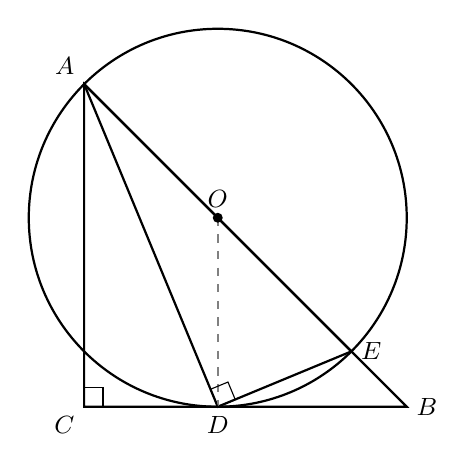
\begin{tikzpicture}[scale=1.2, font=\small]
    % 1. 定义基本参数（圆心和半径）
    \coordinate (O) at (0,0);
    \def\r{2}

    % 2. 定义圆上的点
    % A点在左上方，E点在右下方，AE为直径
    \coordinate (A) at (135:\r);
    \coordinate (E) at (-45:\r);

    % D点是切点，根据题意D在圆周下部。设定D的角度。
    \coordinate (D) at (-90:\r); 

    % 3. 推算其他交点
    % 直线CB是切线，过D点且垂直于半径OD
    % 由于D在正下方，切线CB是水平线
    % C点是过A作AC垂直于CB的垂足
    \coordinate (C) at ($(A)!(D)!(E)$); % 占位计算，实际C在A正下方
    \coordinate (C) at (A |- D); % A的x坐标，D的y坐标

    % B点是直线AE与直线CD(水平线)的交点
    \coordinate (B) at (intersection of A--E and C--D);

    % 4. 绘制图形各部分
    \draw[thick] (O) circle (\r);          % 绘制圆O
    \draw[thick] (A) -- (C) -- (B) -- cycle; % 绘制直角三角形ABC
    \draw[thick] (A) -- (E);                 % 绘制直径AE
    \draw[thick] (A) -- (D) -- (E);          % 绘制弦AD, DE
    \draw[dashed, gray, thick] (O) -- (D);
    % 5. 绘制核心点和标记
    \fill (O) circle (1.5pt) node[above] {$O$};
    \node[above left]  at (A) {$A$};
    \node[below left]  at (C) {$C$};
    \node[below]       at (D) {$D$};
    \node[right]       at (E) {$E$};
    \node[right]      at (B) {$B$};

    % 6. 绘制直角符号
    \tkzMarkRightAngle[size=0.2](A,C,D)    % C处的直角
    \tkzMarkRightAngle[size=0.2](A,D,E)    % D处的圆周角直角

\end{tikzpicture}
\end{document}